% !TeX root = ../main-english.tex
% !TeX spellcheck = en-US
% !TeX encoding = utf8
% -*- coding:utf-8 mod:LaTeX -*-

%This smart spell only works if no changes have been made to the chapter
%using the options proposed in preambel/chapterheads.tex.
\setchapterpreamble[u]{%
	\dictum[Carole Goble]{Better Software, Better Research}
}

%\chapter{Improving scientific practice through software usability: The DataLad Handbook}
\chapter{Improving scientific practice through software usability}
\label{chap:k2}




This next chapter details how a documentation project for DataLad increased software quality, software popularity and enabled users to tackle complex \gls{rdm} use cases.
It refers to our original publication \citet{wagner2020datalad}.


\section{Scientific software}

Scientific software, often also referred to as research software, is an integral part of research in science, engineering, and humanities.
It can broadly be defined as software used for scientific purposes.
As software requirements for scientific use cases can be specialized, the developers of research software often overlap with the community of scientists that uses the software, and over the past decade, the term ``Research Software Engineer'' has been established to describe researchers that dedicate parts of their scientific work to creating and maintaining software \citep{hettrickRSE}



The United Kingdom's Engineering and Physical Sciences Research Council describes software as a ``critical infrastructure that underpins cutting edge science and engineering research'' (CITATION) % https://www.ukri.org/what-we-offer/browse-our-areas-of-investment-and-support/research-infrastructure-theme/

More recently, research software has been gaining academic credit it has long lacked.
It is recognized as academic output in the San Francisco Declaration on Research Assessment (DORA; \href{https://sfdora.org/}{sfdora.org}), and the Agreement on Reforming Research Assessment (CoARA; \href{https://coara.eu}{coara.eu}), both of which have been signed by thousands of academic institutions worldwide. The \gls{grf}, the largest funding institution for the sciences and humanities and research in Germany, counts software a ``scientific result'' in their evaluation of academic CVs.
Academic journals, such as the Journal of Open Source Software (\href{https://joss.theoj.org/}{joss.theoj.org/}), and article types, such as ``Nature Toolbox'' (\href{https://www.nature.com/nature/articles?type=toolbox}{www.nature.com/nature/articles?type=toolbox}), have been created to support the scholarly publication and reuse of research software.
And calls for proposals to improve the quality, usability or longevity of research software have been put forward by major funders, for example in Germany \citep{dfgrs}, the United Kingdom \citep{ukri}, or the United States \citep{nih}.



The largest funding institution for the sciences and humanities and research in Germany, the \gls{grf}, states that access to data and software are of comparable importance to science as access to publications \citep{dfg}

The DFG put forward several timely recommendations: Research software should be open source \citep{dfg}


In an analysis of user questions in support forums of scientific software packages, \citet{swarts2019open} found that the focus in 80\% of inquiries was on operations and tasks, such as a required sequence of operations to achieve a specific goal.
In breaking down user questions by purpose, \citet{swarts2019open} further found that users were most interested in a description of operations or tasks, followed by insights about the reasons behind the action.
And in separating documentation types into ``feature-based'' (closer related to the concept of reference documentation) or ``task-based'' (closer related to the concept of a tutorial),  \citet{swarts2019open} reports twice as many questions seeking explanations in software with feature-based compared to task-based documentation.
This hints at a disconnect between knowing \textit{how} something should be done and \textit{why} it should be done this way.
These results highlight that users of scientific software show a clear need beyond the documentation of individual commands, but seek to understand general usage principles and master complex combinations of features to achieve specified goals.
This type of empowerment is what the DataLad handbook project aimed to achieve.


The high usability of modern computers' and applications' front ends spares users the need to develop the same level of familiarity with their computers than previous generations of computer users had \citep{mehlenbacher2003documentation}.
Only rarely does a consumer tool involve a terminal instead of a \gls{gui}, and typical applications perform a complete suite of tasks such that users do not need to combine several tools to accomplish one goal (CITATION NEEDED).
However, powerful scientific tools are often command-line-based (e.g., EXAMPLES), and complex task sets such as those required in \gls{rdm} require a broad set of technical skills \citep{grisham2016proposed}.
DataLad, too, is primarily developed as a command line tool.

\pagebreak

\section{The DataLad Handbook: A user-focused and workflow-based addition to standard software documentation}

A user-driven alternative to reference documentation by software developers, ``Documentation Crowdsourcing'', has been successfully employed by the NumPy project \citep{pawlik2014crowdsourcing}.
Extending this concept beyond documentation, we have created the DataLad handbook (\href{http://handbook.datalad.org}{handbook.datalad.org}) as a free and open-source, user-driven and -focused narrative tutorial.


Usability adherence

Timeline:
The DataLad Handbook has been under continuous development for more than three years, averaging two releases per year.
As of May 2023, a total of 53 contributors provided input in the form of content, bug fixes, or infrastructure improvements.
During December 2022 and July 2023, the DataLad Handbook averaged 30000 total page views per 30 days.


\begin{figure}
	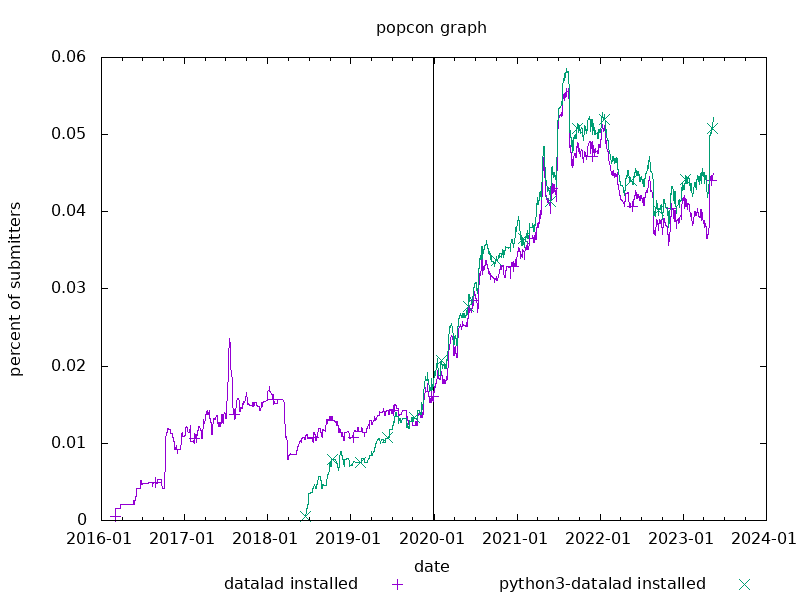
\includegraphics[width=\textwidth]{popcon-datalad.png}
	\caption{d}
	\label{fig:popcon}
\end{figure}

\pagebreak

